
%% Preâmbulo (configurações, pacotes e tudo mais)
%% Preambulo LaTeX: Define classes e características do documento
%% Definição do docuemnto
\documentclass[
	%article,			% Define que este será um artigo (e não uma tese/monografia/relatório)
	12pt,				% Fonte: 12pt
	oneside,			% Impressão: oneside = 1 face, twoside = 2 faces (frente-e-verso)
    %openright,			% capítulos começam em página ímpar (use apenas se usar "twoside")
	a4paper,			% Tamanho do Papel: A4
    chapter=TITLE,		% Todos os capítulos devem ficam em caixa alta
    section=TITLE,		% Todas as seções devem ficar em caixa alta
	english,			% Adiciona Idioma para Hifenização: Inglês
    %spanish,			% Adiciona Idioma para Hifenização: Espanhol
    %french,			% Adiciona Idioma para Hifenização: Francês
	brazil				% Adiciona Idioma para Hifenização: Português do Brasil (o último idioma se torna o principal do documento)
]{abntex2}				% Utilizar ABNTeX2





%% Tipografia
%% Abra este arquivo e selecione uma das opções de fonte nele. A padrão é Times.
%% Tipografia / Fontes
%% AVISO: Todas essas fontes são *bastante semelhantes* aos nomes com as quais as descrevo. Entenda: são iguais, só que oficialmente com outro nome.

%% %%%%%%%%%%%%%%%%%%%%%%%%%%%%%%%%%%%%%%%%%%%%%%%%%%%%% %%
%% Comente todas as outras fontes que você não vai usar! %%
%% %%%%%%%%%%%%%%%%%%%%%%%%%%%%%%%%%%%%%%%%%%%%%%%%%%%%% %%

%% Latin Modern (fonte padrão do LaTeX, Computer Modern, mas com suporte a caracteres acentuados)
%% Considerada a mais clássica e bonita
%\usepackage{lmodern}



%% Times
%% Considerada a mais confortável de ler quando impresso
%%\usepackage{mathptmx}

%% Variação da mesma fonte, com minúsculas diferenças entre uma e outra (coisas bastante técnicas como kerning, aliasing e afins) - Essa tem revisões frequentes
%\usepackage{newtxtext} \usepackage{newtxmath}



%% Arial
%% Considerada mais confortável de ler num computador
%% ** Oficialmente recomendada pelo manual de formatação do IFPI **
\usepackage{helvet} \renewcommand{\familydefault}{\sfdefault}



%% Palatino
%% Uma opção mais elegante à Times
%\usepackage{newpxtext}



%% Kepler
%% Variação evoluída da Palatino, com várias pequenas diferenças e refinamentos
%\usepackage{kpfonts}



%% Libertine
%% Uma fonte estilo Serif comum no Linux
%\usepackage{libertine} %\usepackage[libertine]{newtxmath}



%% Pacotes usados pelo documento (se não entender não mexa, hehehe)
\usepackage{courier}                    % Permite a utilização da fonte Courier (para códigos-fonte)
\usepackage[T1]{fontenc}				% Seleção de códigos de fonte.
\usepackage[utf8]{inputenc}				% Codificação do documento (conversão automática dos acentos)
\usepackage{indentfirst}				% Indenta o primeiro parágrafo de cada seção.
\usepackage{nomencl} 					% Usado pela Lista de símbolos
\usepackage{color}						% Controle das cores
\usepackage{graphicx}					% Inclusão de gráficos
\usepackage{float}						% Melhorias para posicionamento de gráficos e tabelas
\usepackage{microtype} 					% Melhorias na justificação
\usepackage{lastpage}   		        % Dá acesso ao número da última página do documento
\usepackage{booktabs}					% Comandos para tabelas
\usepackage{multirow, array}			% Múltiplas linhas e colunas em tabelas
\usepackage{titlesec}                   % Permite criar múltiplas sub seções
\usepackage[table,xcdraw]{xcolor}       % Cores para algumas tabelas especiais
\usepackage[brazilian,hyperpageref]{backref}	 % Inclui nas Referências as páginas onde há as citações
\usepackage{simplecd}                   % Pacote para gerar capa do CD
\usepackage[final]{pdfpages}            % Pacote para incluir um PDF dentro de outro (ficha catalográfica)



%% Adiciona as alterações do ABNTeX-IFFar
\usepackage{abntex-iffar/abntex-iffar}

% Modificações do ABNTeX para o IFPI
\usepackage{abntex-iffar/tikz-uml}	    % Pacote Tikz UML para criar UML no LaTeX





%% Metadados
%% Configurações dos metadados do PDF
\makeatletter
\hypersetup{
  pdftitle={\@title}, 
  pdfauthor={\@author},
  pdfsubject={\@title},
  pdfcreator={LaTeX, abntex2, {abnTeX\-ifpi}},
  %% Coloque aqui suas palavras-chave, cada uma entre chaves: {palavra}{palavra}{outra palavra}...
  pdfkeywords={palavra 1}{palavra 2}{palavra 3}{palavra 4}{palavra 5},
  colorlinks=true,			% Visual dos Links: false = caixas; true = colorido
  linkcolor=cor-link,		% Cor dos Links Internos (preto)
  citecolor=cor-link,		% Cor de Links para Bibliografia (preto)
  filecolor=cor-link,		% Cor para Links a Arquivos (preto)
  urlcolor=cor-link,		% Cor para Links a URLs (preto)
  bookmarksdepth=4
}
\makeatother



%% Metadados
%% %%%%%%%%%%%%%%%%%%%%%%%%%%%%%%%%%%%%%%%%%%%%%%%% %%
%% Metadados do trabalho
%% AVISO: Todos esses dados serão automaticamente convertidos para caixa alta onde necessário
%% %%%%%%%%%%%%%%%%%%%%%%%%%%%%%%%%%%%%%%%%%%%%%%%% %%

%% Título
\titulo{Sistema V. Tornos: Solução Web para Orçamentos e Serviços em Manutenção de Maquinários agrícola e pecuária}

%% Autor
\autor{Vagner Roballo Garcia}

%% Nome do Curso (usado para a Capa do CD)
\nomedocurso{Bacharelado em Sistemas de Informação}

%% Local de publicação
\local{São Borja, Rio Grande do Sul}

%% Preâmbulo do trabalho
\preambulo{Trabalho de Conclusão de Curso (monografia) apresentado como exigência parcial para obtenção do diploma do Curso de Bacharelado em Sistemas de Informação do Instituto Federal de Educação, Ciência e Tecnologia Farroupilha, Campus São Borja.}

%% Orientador
%% "M\textsuperscript{e}." = Abreviação oficial para "Mestre"
\orientador{Prof. Dr. Fernando Luis de Oliveira}
\coorientador{Prof. Dr. Rafael Baldiati Parizi}

%% Tipo de Trabalho
%% - Monografia
%% - Tese (Mestrado)
%% - Tese (Doutorado)
%% - Relatório técnico
\tipotrabalho{Monografia}

%% Data do Trabalho
\data{2024}

%% Nome da Instituição (para a capa)
\instituicao{INSTITUTO FEDERAL DE EDUCAÇÃO, CIÊNCIA E TECNOLOGIA FARROUPILHA
\\
CAMPUS SÃO BORJA
\\
BACHARELADO EM SISTEMAS DE INFORMAÇÃO}

%% Primeiro membro da banca examinadora
\membroum{Prof. Dr. Claiton Correa}

%% Segundo membro da banca examinadora
\membrodois{Prof. Ms. Icaro Lins Iglesias}

%% Terceiro membro da banca examinadora
%\membrotres{Prof. Dr. Xxxxxx Xxxxx}

%% Data da apresentação do trabalho
%% Se não souber a data da apresentação, utilize \underline{\hspace{3.5cm}}
%% Isso cria um sublinhado de 3.5cm, onde você pode escrever a data depois!
%\dataapresentacao{02 de Outubro de 2023}
\dataapresentacao{\underline{\hspace{1.0cm}}/\underline{\hspace{1.0cm}}/\underline{\hspace{1.75cm}}}



%% Configuração do "Citado nas páginas"
%% Configuração das Citações

%% Estilo
%\usepackage[num]{abntex2cite}			% Citações numéricas
\usepackage[alf, 
 versalete, 
 abnt-emphasize = bf, 
abnt-etal-list = 3,
abnt-etal-text = it, 
abnt-and-type = &, 
abnt-last-names = abnt, 
abnt-repeated-author-omit = no  '____.']{abntex2cite}			% Citações "AUTOR, ano"

% Definição do negrito

%% Colocar entre parênteses ou colchetes?
%% Padrão: Parênteses
%% * Fica mais agradável usar colchetes quando se usa citações numéricas
%\citebrackets[]							% Comente essa linha e o documento usará parênteses


%% Configura o "Citado nas Páginas ..." nas referências
%% Não mexa nesse:
\renewcommand{\backref}{}

%% Esse é o texto do "Citado nas páginas ..."
\renewcommand*{\backrefalt}[4]{
	\ifcase #1
		Nenhuma citação no texto.
	\or
		Citado na página #2.
	\else
		Citado #1 vezes nas páginas #2.
	\fi}



%% Cores
%% Cores do Documento

%% Cor dos Links do PDF
%% Usando preta você "esconde" os links
\definecolor{cor-link}{RGB}{0,0,0}

%% Usando azul os links ficam visíveis (ruim para impressão)
%\definecolor{cor-link}{RGB}{8,40,75}



%% Cor para os quadros
%% Dê preferência a cores escuras.
%% Boa referência para cores: https://material.io/guidelines/style/color.html#color-color-palette
\definecolor{cor-quadro}{RGB}{5,28,63}		% Azul Escuro



%% Espaçamentos
%% Espaçamentos
%% O tamanho do parágrafo é dado por:
\setlength{\parindent}{1.5cm}

%% Espaçamento entre um parágrafo e outro:
%% O abntex diz: "tente também \onelineskip"
\setlength{\parskip}{0cm}


%% Início do Documento
\begin{document}

%% Documento será escrito em Português do Brasil
\selectlanguage{brazil}

%% Elementos pré-textuais: capa, folha de rosto, dedicatória, listas, sumário, etc.
%% %%%%%%%%%%%%%%%%%%%%%%%%%%%%%%%%%%%%%%%%% %%
%% Elementos Pré Textuais
%% ----------------------
%% 
%% Segundo o manual do IFPI, eles devem ser os seguintes (nessa ordem):
%%  1. Capa (obrigatório)
%%  2. Folha de rosto (obrigatório)
%%  3. Errata (opcional)
%%  4. Folha de aprovação (obrigatório)
%%  5. Dedicatória (opcional)
%%  6. Agradecimentos (opcional)
%%  7. Epígrafe (opcional)
%%  8. Resumo (obrigatório)
%%  9. Abstract/Resumo em outra língua (obrigatório)
%% 10. Lista de Ilustrações (opcional)
%% 11. Lista de Tabelas (opcional)
%% 12. Lista de Abreviaturas e Siglas (opcional)
%% 13. Lista de Símbolos (opcional)
%% 14. Sumário (obrigatório)
%% %%%%%%%%%%%%%%%%%%%%%%%%%%%%%%%%%%%%%%%%% %%

%% 01: Capa
\imprimircapa



%% 02: Folha de Rosto
%% OBS: O asterisco indica que haverá ficha bibliográfica (só funciona para impressão frente-e-verso)
\imprimirfolhaderosto*



%% Ficha Catalográfica (acho que é melhor adicionar via \includepdf depois)
%% Ficha Catalográfica
%%
%% Este template cria um quadro semelhante a ficha catalográfica oficial.
%% É melhor usar \includepdf depois que a ficha oficial estiver em mãos.


% 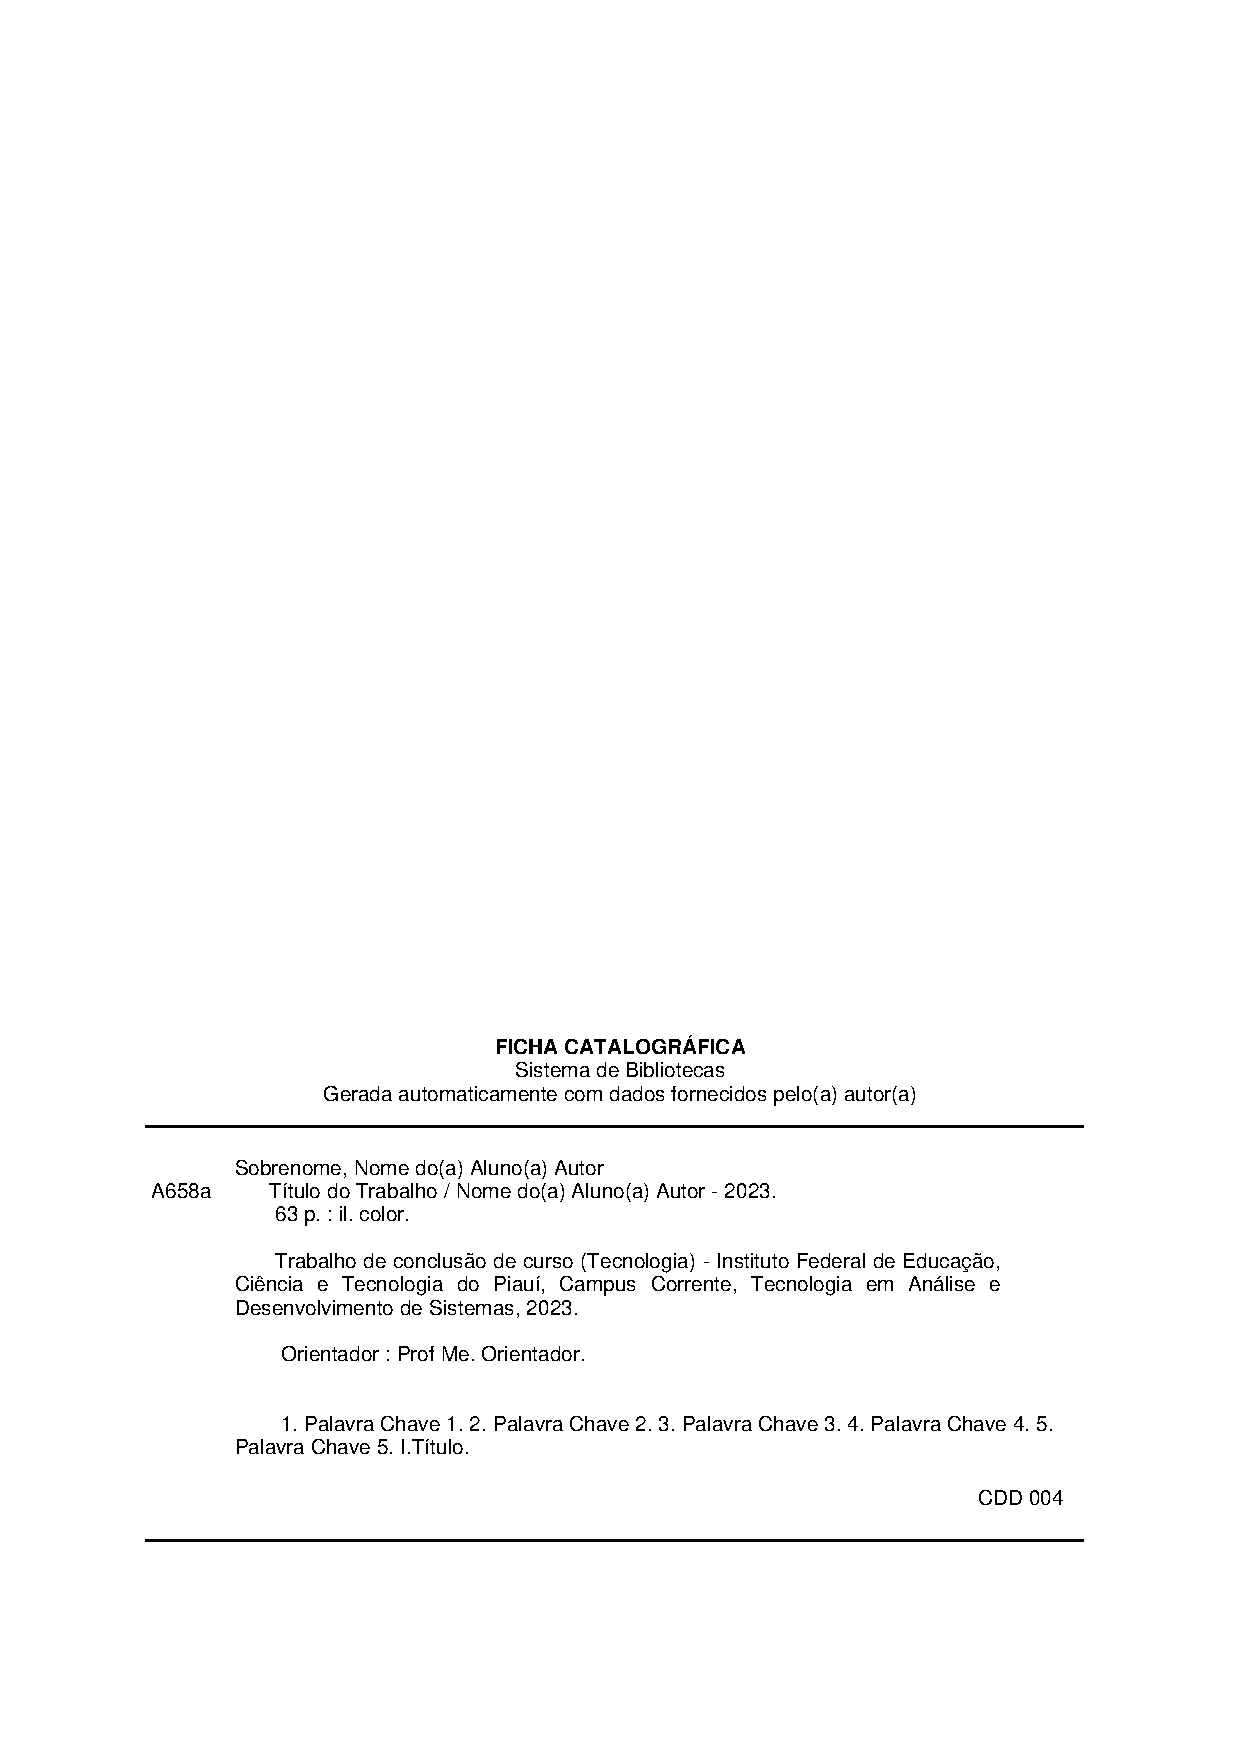
\includepdf{pre-textual/ficha-catalografica.pdf}

%% Caso queira fazer a ficha "tradicional" (este serve apenas como um modelo)
%\begin{fichacatalografica}
%	\sffamily
%	\vspace*{\fill}					% Posição vertical
%	\begin{center}					% Minipage Centralizado
%	\fbox{\begin{minipage}[c][8cm]{13.5cm}		% Largura
%	\small
%	\imprimirautor
%	
%	\hspace{0.5cm} \imprimirtitulo  / \imprimirautor. --
%	\imprimirlocal, \imprimirdata-
%	
%	\hspace{0.5cm} \thelastpage p. : il. (algumas color.) ; 30 cm.\\
%	
%	\hspace{0.5cm} \imprimirorientadorRotulo~\imprimirorientador\\
%	
%	\hspace{0.5cm}
%	\parbox[t]{\textwidth}{\imprimirtipotrabalho~--~\imprimirinstituicao,
%	\imprimirdata.}\\
%	
%	\hspace{0.5cm}
%		1. Palavra-chave1.
%		2. Palavra-chave2.
%		2. Palavra-chave3.
%		I. Orientador.
%		II. Universidade xxx.
%		III. Faculdade de xxx.
%		IV. Título 			
%	\end{minipage}}
%	\end{center}
%\end{fichacatalografica}


%% 03: Errata
%% Errata
%\begin{errata}
%Elemento opcional da norma ABNT NBR14724 de 2011. Exemplo:
%
%\vspace{\onelineskip}
%
%FERRIGNO, C. R. A. \textbf{Tratamento de neoplasias ósseas apendiculares com reimplantação de enxerto ósseo autólogo autoclavado associado ao plasma rico em plaquetas}: estudo crítico na cirurgia de preservação de membro em cães. 2011. 128 f. Tese (Livre-Docência) - Faculdade de Medicina Veterinária e Zootecnia, Universidade de São Paulo, São Paulo, 2011.

%% Tabela de exemplo com os erros
%\begin{table}[htb]
%\center
%\footnotesize
%\begin{tabular}{|p{1.4cm}|p{1cm}|p{3cm}|p{3cm}|}
%  \hline
%   \textbf{Folha} & \textbf{Linha}  & \textbf{Onde se lê}  & \textbf{Leia-se}  \\
%    \hline
%    1 & 10 & auto-conclavo & autoconclavo\\
%   \hline
%\end{tabular}
%\end{table}
%
%\end{errata}



%% 04: Folha de Aprovação
\imprimirfolhadeaprovacao
%% Use esta se forem 4 membros na banca:
%\imprimirfolhadeaprovacaoduascolunas



%% 05: Dedicatória
%% Dedicatória do seu trabalho
\begin{dedicatoria}
	%% Empura o texto a seguir para a parte de baixo da página
	\vspace*{\fill}
    
    %% Alinhado a Direita
    \center
    \begin{flushright}
    	Dedico este trabalho a todos que acreditaram que ele sairia.
    \end{flushright}
    
    %% Descomente a linha seguir para deixar o texto centralizado verticalmente na página
    %% Lembre de comentar o "\begin{}" e "\end{}" acima para centralizar o texto da dedicatória.
	%\vspace*{\fill}
\end{dedicatoria}



%% 06: Agradecimentos
%% Agradecimentos
\begin{agradecimentos}
Agradeço a todos os professores e servidores do IFFar do Campus São Borja, pois todos xxxxxxxxxxxxxxxxxxxxxxxxxxxxxxx. Xxxxxxxxxxxxxxxxxxx, que deu todo o apoio necessário para que chegasse até aqui. Agradeço ao meu Deus, que me deu força quando mais precisava.
\end{agradecimentos}



%% 07: Epígrafe
%% Epígrafe
%% Uma frase que lhe inspira ou a qual lhe inspirou a fazer este trabalho
\begin{epigrafe}
\vspace*{\fill}
\begin{flushright}
\emph{"Existe um tempo para ousadia e um tempo para cautela, e o homem sábio sabe o momento de cada um deles." 
  \\ \textbf{Sociedade dos poetas mortos} -- 1989}
\end{flushright}
\end{epigrafe}



%% 08: Resumo
%% Resumo
\begin{resumo}
Apresentação concisa dos pontos relevantes do documento. Deve Informar ao leitor 
finalidades, metodologia, resultados e conclusões do documento, de tal forma que 
este possa, inclusive, dispensar a consulta ao original. Deve-se usar o verbo na voz 
ativa e na terceira pessoa do singular, contendo de 150 a 500 palavras. O resumo 
deve ser composto de uma sequência de frases concisas, afirmativas e não de 
enumeração de tópicos. Recomenda-se o uso de parágrafo único, mesma fonte do 
trabalho, e espaçamento entrelinhas 1,5. Resumo resumo resumo resumo resumo 
resumo resumo resumo resumo resumo resumo resumo resumo resumo resumo 
resumo resumo resumo resumo resumo resumo resumo resumo resumo resumo 
resumo resumo resumo resumo resumo resumo resumo resumo resumo resumo 
resumo ( ASSOCIAÇÃO BRASILEIRA DE NORMAS TÉCNICAS, 2021).
\vspace{\onelineskip}
\noindent

\textbf{Palavras-chaves}: Palavra 1; Palavra 2; 
Palavra 3.
\end{resumo}

%% 09: Abstract/Resumo em língua estrangeira
%% Abstract (configurado para língua inglesa)
\begin{resumo}[Abstract]			% Título do Resumo (Abstract = Resumo em inglês)
\begin{otherlanguage*}{english}		% Língua do texto
Elemento obrigatório, com as mesmas características do resumo em língua 
vernácula, digitado em folha separada (em inglês Abstract, em espanhol Resumen, 
em francês Résumé, por exemplo). Abstract abstract abstract abstract abstract 
abstract abstract abstract abstract abstract abstract abstract abstract abstract 
abstract abstract abstract abstract abstract abstract abstract abstract abstract 
abstract abstract abstract abstract abstract abstract abstract abstract abstract 
abstract abstract abstract. ( ASSOCIAÇÃO BRASILEIRA DE NORMAS TÉCNICAS, 2021). 

\vspace{\onelineskip}
\noindent
\textbf{Keywords}: Word 1; Word 2; Word 3.
\end{otherlanguage*}
\end{resumo}

%% Exemplo de resumo em francês
%\begin{resumo}[Résumé]
% \begin{otherlanguage*}{french}
%    Il s'agit d'un résumé en français.
% 
%   \textbf{Mots-clés}: latex. abntex. publication de textes.
% \end{otherlanguage*}
%\end{resumo}

%% Exemplo de resumo em Espanhol
%\begin{resumo}[Resumen]
% \begin{otherlanguage*}{spanish}
%   Este es el resumen en español.
%  
%   \textbf{Palabras clave}: latex. abntex. publicación de textos.
% \end{otherlanguage*}
%\end{resumo}
% ---



%% 10: Lista de Ilustrações
%% Lista de Ilustrações
\pdfbookmark[0]{\listfigurename}{lof}
\listoffigures*
\cleardoublepage



%% 11: Lista de Tabelas
%% Lista de Tabelas
%\pdfbookmark[0]{\listtablename}{lot}
%\listoftables*
%\cleardoublepage



%% 12: Lista de Abreviaturas e Siglas
%% Lista de Siglas
\begin{siglas}
  \item[ABNT] Associação Brasileira de Normas Técnicas
  \item[CRB] Conselho Regional de Biblioteconomia
  \item[IBGE] Instituto Brasileiro de Geografia e Estatística
  \item[IFFar] Instituto Federal Farroupilha
\end{siglas}



%% 13: Lista de Símbolos
%% Lista de Símbolos
%% (esta é apenas uma lista de exemplo)
\begin{simbolos}
  \item [\% ] Porcentagem
  \item [ © ] Copyright
  \item [ ® ] Marca registrada
  \item [ \$ ] Dólar
  \item [ § ] Seção
  \item[$ \Gamma $] Letra grega Gama
  \item[$ \Lambda $] Lambda
  \item[$ \zeta $] Letra grega minúscula zeta
  \item[$ \in $] Pertence
\end{simbolos}



%% 14: Sumário (o asterisco retira o próprio sumário do sumário)
\pdfbookmark[0]{\contentsname}{toc}
\tableofcontents*
\cleardoublepage



%% Indica que a partir daqui ficarão os elementos textuais (TCC em si)
\textual

%% Inclui os capítulos do TCC (parte textual)
%% %%%%%%%%%%%%%%%%%%%%%%%%%%%%%%%%%%% %%
%% Elementos Textuais (Capítulos)      %%
%% %%%%%%%%%%%%%%%%%%%%%%%%%%%%%%%%%%% %%
\pagestyle{empty} % Remover cabeçalho com titulo dos capítulos
%% Inclua aqui os capítulos que farão parte do TCC
% ----------------------------------------------------------
% Introdução
% ----------------------------------------------------------
\chapter{Introdução}\label{sec:Introdução}

A tecnologia da informação está presente em todos os segmentos da sociedade, abrangendo desde o lazer até diversas atividades e serviços. Dessa forma, sua utilização proporciona ganhos significativos em conhecimento, reduz o tempo necessário para encontrar soluções e esclarece quais passos e produtos podem resolver problemas específicos. Assim, aqueles que utilizam a tecnologia da informação ganham notoriedade por sua eficiência e eficácia \mbox{\cite{a:gestao_inovacao_2024}.}

 Assim é essencial que as empresas estejam sempre aprimorando suas atividades para aumentar a produtividade e se destacar no mercado. Nesse contexto, a implementação de Sistemas de Informação (SI), desempenha um papel fundamental, permitindo a análise rápida de cenários e ajudando a empresa a otimizar suas operações mais relevantes \mbox{\cite{a:tecnologia_empresa_2024}.}

De fato, o setor de administração e gestão deve possuir um profundo conhecimento e compreensão das informações geradas pelas atividades do negócio. Não há espaço para ``achismos'' ou uma condução amadora da empresa, pois, se os responsáveis pela gestão não prestarem a devida atenção nas etapas e ciclos que compõem seu ramo de atividade, a probabilidade de perder oportunidades e até mesmo enfrentar a falência aumenta consideravelmente \mbox{\cite{b:administracao_gestao_2024}}. Ao analisar o cenário, é possível neutralizar ou minimizar potenciais riscos. Além disso, um obstáculo pode ser transformado em uma oportunidade quando identificado com antecedência, graças a uma gestão eficaz que utiliza a tecnologia da informação e demonstra interesse em inovar \mbox{\cite{a:gestao_inovacao_2024}}.

A empresa V Tornos é uma microempresa de capital limitado com mais de cinco anos de experiência no mercado, especializada na manutenção de equipamentos agrícola e pecuária. Sendo um negócio familiar, ela desenvolve suas atividades documentais utilizando blocos de notas e planilhas de Excel para organizar e registrar suas operações. Dessa forma, a implementação de um sistema informatizado de gestão documental para suas operações e administração se torna crucial para possibilitar futuras expansões e otimizações no segmento em que atua.

Este projeto tem como objetivo desenvolver um sistema de suporte a orçamentos e serviços que gere informações sobre quais equipamentos apresentam o maior número de reparos. Dessa forma, a implementação de um software tem como objetivo inovar a empresa V Tornos, atualizando a documentação das operações para enfrentar os desafios e aproveitar as oportunidades no dinâmico segmento de manutenção em usinagem. Neste contexto, é fundamental desenvolver a capacidade de explorar novas oportunidades, integrar conhecimentos, utilizar recursos internos e externos, e estar em constante aperfeiçoamento e adaptação para às mudanças e incertezas do mercado.


Este trabalho está organizado da seguinte forma: a Seção \ref{sec:justificativa} apresenta a justificativa; a Seção \ref{sec:problema} especifica o cenário onde o software implementará as melhorias; a Seção \ref{sec:objetivo} delineia as intervenções da aplicação; a Seção \ref{sec:fundamentacao} aborda a história da industrialização, tipos de manutenção, conceitos de usinagem e breve contextualização sobre sistemas web; a Seção \ref{sec:metodologia} apresenta o modelo de caso de uso e o diagrama de Entidade Relacionamento com as tabelas do banco de dados; e, por fim, a última seção apresenta o cronograma de desenvolvimento de cada atividade.

\section{Justificativa}\label{sec:Justificativa}

A empresa V. Tornos é uma microempresa que oferece serviços no setor de maquinário para agricultura e pecuária. Suas atividades envolvem usinagem para reparos parciais ou fabricação de peças novas em situações de avarias graves que requerem substituição. De modo que as peças são reparadas ou fabricadas artesanalmente, seguindo medidas precisas para atender às dimensões da máquina e garantir o funcionamento correto das partes do equipamento. Adicionalmente, os clientes costumam solicitar serviços de adaptação para melhorar o desempenho ou prolongar a vida útil das peças sujeitas ao desgaste devido ao uso constante.

A empresa, conforme ilustrado na Figura \ref{fig:diagrama_VTornos}, adota um processo estruturado para realizar a manutenção de peças e equipamentos. O processo inicia com uma inspeção, que inclui a desmontagem dos componentes para identificar avarias ou desgastes. Em seguida, uma análise dos componentes é conduzida. Baseado nos resultados, é feito uma classificação para determinar o grau de desgaste e as causas das falhas, criando uma documentação apropriada para futuras referências. Com essas informações, um plano de manutenção é desenvolvido, detalhando as ações necessárias, como reparos ou substituições, e essa proposta é comunicada ao cliente. A manutenção é então executada após a aprovação, ou o equipamento é devolvido caso o cliente opte por não realizar a reparação com a V Tornos.

\begin{figure}[htb!]
    \centering
    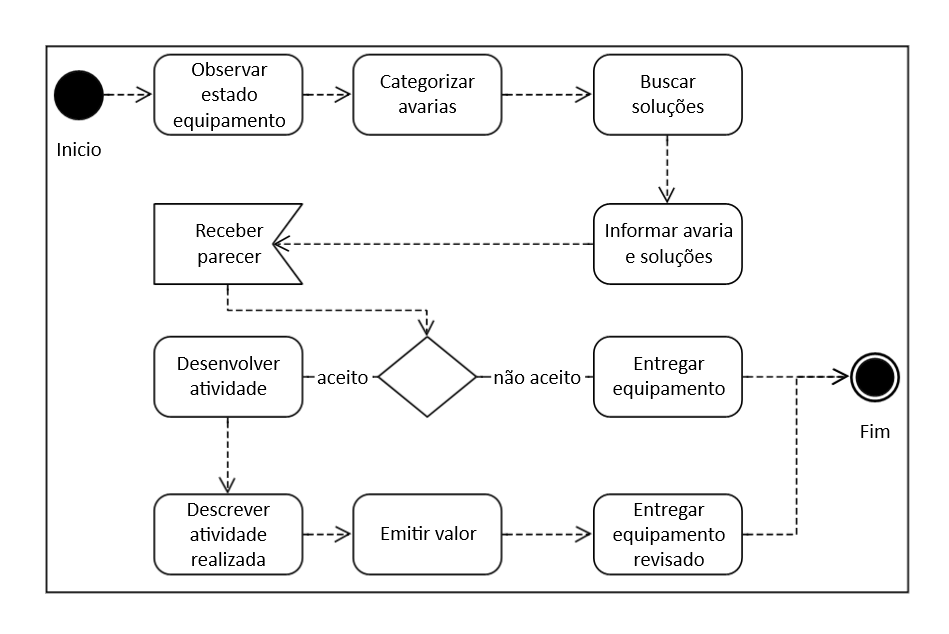
\includegraphics[width=.75\linewidth]{figs/diagrama_atividade_VTornos.png}
    \caption{Passos da V Tornos para realizar manutenção de peça ou equipamento}
    \label{fig:diagrama_VTornos}
\end{figure}

Dessa forma, a empresa tem como objetivo central a manutenção, pois desenvolve peças para situações específicas conforme os parâmetros dos maquinários já com tempo de uso. Isso a diferencia de uma empresa de produção industrial, onde existe um modelo computacional já pronto para uso e um cronograma mensal definindo quais peças serão produzidas em tornos automatizados, sem produção de peças fora do padrão estabelecido.

A proposta para este trabalho inclui a implementação de um sistema de orçamentos para a V. Tornos, levando em consideração os requisitos para a prestação de serviços. É fundamental manter um equilíbrio entre as operações e inovações para garantir uma administração saudável, de forma a aproveitar as oportunidades do mercado. O sistema permitirá visualizar quais atividades estão sendo mais desenvolvidas, auxiliando na tomada de decisões e na identificação de áreas de foco para o crescimento da empresa.

\section{Objetivos}

As finalidades do trabalho são pontuadas a partir das seguintes questões, conforme descrito nas subseções geral e específicos.

\subsection{Geral}\label{sec:objGeral}

Desenvolver sistema de gestão de orçamento e serviços para melhoria operacional e administrativa da empresa V. Tornos.

\subsection{Objetivos Específicos}\label{sec:objEspc}

\begin{itemize}
   \item Melhorar a gestão de dados dos cliente e respetivas inscrições municipais e estaduais;
   \item Manter registros de serviços já prestados para futuras consultas;
   \item Facilitar o controle de insumos ofertados para os clientes;
   \item  Gerar relatórios e dashboards específicos para tomada de decisões empresariais.
\end{itemize}
% ----------------------------------------------------------
% Fundamentação Teórica
% ----------------------------------------------------------
\chapter{Fundamentação Teórica}
\label{cha:fundamentacao}

Nesta seção apresenta o referencial teórico relacionado às peculiaridades necessárias para o desenvolvimento de um sistema web com seu objetivo. É importante destacar que esse modelo pode ser hospedado fora do ambiente físico da empresa, permitindo o acesso por usuários devidamente cadastrados. Dessa forma, o sistema pode ser utilizado enquanto houver uma conexão de internet adequada para sua operação.

\section{História da industrialização}
\label{sec:hist_industria}

A humanidade sempre buscou desenvolver ferramentas desde os primórdios com o objetivo de facilitar o trabalho e realizando manutenções conforme o necessário. É importante ressaltar que, ao longo do tempo, essas ferramentas rudimentares passaram por aperfeiçoamentos, resultando em utensílios mais específicos que visam aprimorar as atividades realizadas. No entanto, a precisão e a padronização só começaram a surgir a partir da Revolução Industrial.

De modo que a indústria encontra-se em sua quarta geração, conforme ilustrado na Figura \ref{fig:etapas_industria}. Assim, a manutenção deve estar sempre alinhada às atualizações da versão industrial, pois precisa fornecer o suporte técnico necessário para solucionar defeitos nos maquinários. A primeira versão de manutenção é conhecida como ``manutenção corretiva sem planejamento", onde as intervenções são limitadas a rotinas básicas, como a troca de peças com avarias por desgaste ou quebra, além de limpezas e lubrificações. Vale ressaltar que as máquinas só paravam quando apresentavam um defeito que as tornava inoperantes em realizar a atividade \mbox{\cite{a:manutencao_industriav4_2023}.}

\begin{figure}[th!]
    \centering
    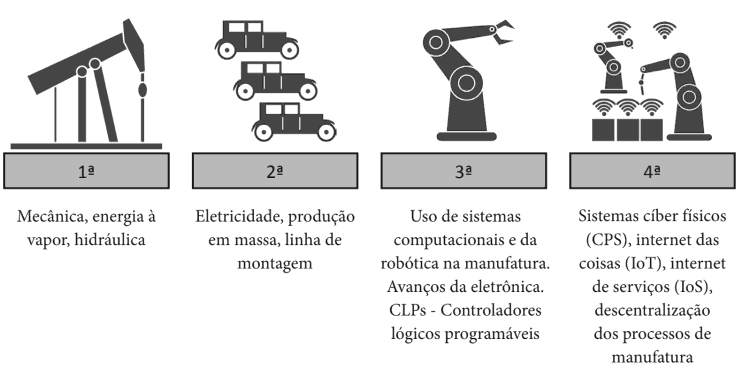
\includegraphics[width=0.75\linewidth]{figs/industria_as_4_versoes.png}
    \caption{Ilustração sobre as versões da indústria \cite{b:industria_v4_2018}}
    \label{fig:etapas_industria}
\end{figure}

A segunda fase concentrou-se na manutenção preventiva. Nesse contexto, surgiram os primeiros sistemas de planejamento e controle de manutenção, que se tornaram componentes essenciais da manutenção moderna, especialmente por razão das duas Guerras Mundiais. Muitas empresas implementaram planos de desenvolvimento na produção, impulsionadas pela necessidade de manter seus maquinários em condições aceitáveis para desempenhar suas funções. Além disso, as indústrias começaram a buscar maneiras de prolongar a vida útil de seus produtos, visando fidelizar os clientes em resposta ao aumento dos custos. Modelos como fordismo, toyotismo e taylorismo passaram a ganhar destaque.

 De acordo com a análise realizada por \mbox{\citeonline{a:manutencao_industriav4_2023},} a terceira fase da indústria pode ser caracterizada pelos seguintes tópicos.
 \begin{itemize}
     \item \textbf{Just-in-Time (JIT)}: Esse método contribui para a redução do desperdício e a melhoria da eficiência, assegurando que os materiais cheguem na hora e na quantidade adequadas, evitando excessos de estoque. Para isso, é essencial um planejamento logístico eficaz e uma colaboração estreita com os fornecedores, sendo os contratos fundamentais para a formalização dessa parceria.

     \item \textbf{Impactos da Paralisação}: As interrupções na cadeia de suprimentos podem impactar negativamente tanto a qualidade quanto os custos de produção. Ressaltando a importância de elaborar planos de contingência e estratégias eficazes de gerenciamento de riscos, a fim de evitar a perda de desempenho e garantir que as demandas planejadas sejam atendidas de maneira adequada.

     \item \textbf{Segurança}: A segurança é uma preocupação fundamental, e as empresas devem cumprir normas e legislações rigorosas que visam proteger os colaboradores. A adoção de práticas seguras não apenas promove um ambiente de trabalho mais protegido, mas também contribui para a melhoria da moral da equipe e eleva a produtividade.

     \item \textbf{Legislação Ambiental}: O aumento da atenção às questões ambientais tem impulsionado as organizações a adotar práticas sustentáveis, como a redução de resíduos e o uso eficiente dos recursos naturais. Essas iniciativas não apenas proporcionam benefícios econômicos, mas também melhoram a imagem corporativa das empresas na sociedade.

     \item \textbf{Informática na indústria}: A adoção de sistemas contribui para aumentar a confiabilidade na produção, permitindo a implementação de manutenção preditiva, que utiliza estatísticas para prever possíveis falhas. Com testes realizados sob supervisão, é possível obter métricas que indicam quando é necessária uma intervenção, minimizando assim o tempo de parada do maquinário.  
 \end{itemize}

A quarta versão da indústria pode ser caracterizada como uma atualização significativa da terceira. Durante a terceira versão, observou-se uma falha de comunicação entre os setores de engenharia, manutenção e operações, resultando em uma elevada taxa de produtos manufaturados com defeitos precoces. Nessa fase, a manutenção era tratada como um mecanismo reativo para corrigir falhas. Em contrapartida, a quarta versão da indústria propõe uma abordagem preventiva, visando minimizar ao máximo a ocorrência de problemas \mbox{\cite{a:manutencao_industriav4_2023}.} De modo, essa nova abordagem estimula o compartilhamento de soluções e estratégias para lidar com avarias, aproveitando os avanços em tecnologia da informação e utilização de redes, que promovem uma comunicação mais eficaz e segura \mbox{\cite{a:osi_tcpip_2024}.}

\section{Tipos de manutenções}
\label{sec:tipos_manutencao}

Está seção aborda as categorizações dos tipos de manutenções que o referencial teórico explora, conforme os seguintes itens:

\subsection{Manutenção corretiva planejada}
\label{sub:manutencao_corretiva_planejada}

Trata-se de manutenções corretivas planejada, nas quais existe uma métrica que mensura quanto tempo de operação que uma peça pode suportar antes de comprometer a integridade do grupo ou por completo do maquinário, enfatizando a necessidade de cuidados durante a operação. Nesse contexto, o objetivo é planejar paradas programadas do maquinário e monitorar quais operações e cargas foram aplicadas durante um determinado período de trabalho. Para isso, é adotado um agendamento prévio para a manutenção, que permite monitorar o grau de desgaste das peças e identificar quais reparos e substituições são necessários. É importante ressaltar que a perda total de um maquinário pode ocorrer se essas manutenções não forem realizadas corretamente.

\subsection{Manutenção corretiva não planejada}
\label{sub:manutencao_corretiva_nao_planejada}

Trata-se de manutenções que ocorrem devido a falhas imprevistas, sem um planejamento pré-estabelecido. Essas falhas podem resultar de descuidos ou do uso excessivo do maquinário em atividades ou ainda da utilização de peças que já apresentam desgaste. Esse tipo de manutenção gera uma série de desafios logísticos, uma vez que o problema pode demandar a aquisição de várias peças que talvez não estejam disponíveis para o reparo que será realizado.

\subsection{Manutenção preventiva}
\label{sub:manutencao_preventiva}

Trata-se de manutenções rotineiras que têm como objetivo monitorar os parâmetros e realizar pequenos ajustes, por exemplo verificar os níveis de água e óleo, completando-os quando estão abaixo do recomendado. Essas manutenções visam identificar irregularidades que, se não corrigidos, podem resultar em falhas graves. Além disso, não é necessário ser um especialista para realizar essas intervenções, pois elas estão sempre documentadas nos manuais de instruções do maquinário.

\subsection{Manutenção preditiva}
\label{sub:manutencao_preditiva}

Estes são tipos de manutenção que permitem a detecção antecipada de problemas, exigindo um olhar especializado para identificar situações que possam resultar em falhas futuras com uso software para analise de dados. A monitoração dos parâmetros de condição e desempenho dos equipamentos deve ser contínua, pois essas características são essenciais para prever o que pode ocorrer em determinadas circunstâncias. Conceito de sensores de falhas são implementados de modo primário.

\subsection{Manutenção prescritiva}
\label{sec:manutencao_prescritiva}

A manutenção prescritiva é uma evolução da manutenção preditiva. Esse método busca integrar ferramentas e sistemas da manutenção preditiva com técnicas de mineração de dados, utilizando algoritmos e modelos matemáticos para sugerir as melhores possibilidades de intervenção na manutenção. O objetivo é evitar paradas da máquina durante os períodos de maior demanda nas atividades de produção.

\section{Usinagem}
\label{sec:usinagem}

A usinagem é um processo fundamental na fabricação de peças, pois transforma insumos de diversos, como madeira, alumínio, nylon, aço e bronze, em produtos manufacturados. Esse processo utiliza ferramentas para remover o material em excesso, conhecido como desbaste, que gera cavacos, até que a peça atinja as dimensões desejadas do projeto, podendo em conjunto com outras peças formarem um equipamento por completo \mbox{\cite{a:guia_usinagem_2024}.}

Dessa forma, o torno é uma ferramenta que, embora simples, apresenta complexidade, pois opera em dois eixos: transversal e longitudinal conforme a Figura \ref{fig:tornos} contém um modelo mecânico manual e um computadorizado. Vale ressaltar para a operação desses maquinários é necessário utilizar API proteção individual como abafadores ruídos, óculos protetor ocular ou mascara protetora facial, luvas, roupas e botinas adequadas para operação.

\begin{figure}[tbh!]
    \centering
    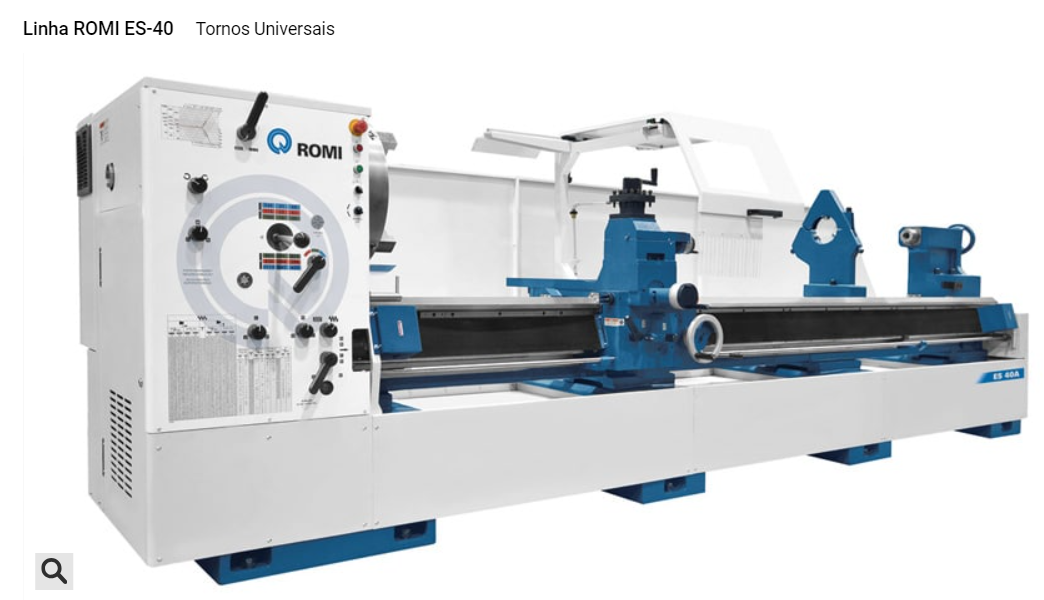
\includegraphics[width=0.48 \linewidth]{figs/rome_es40.png}
    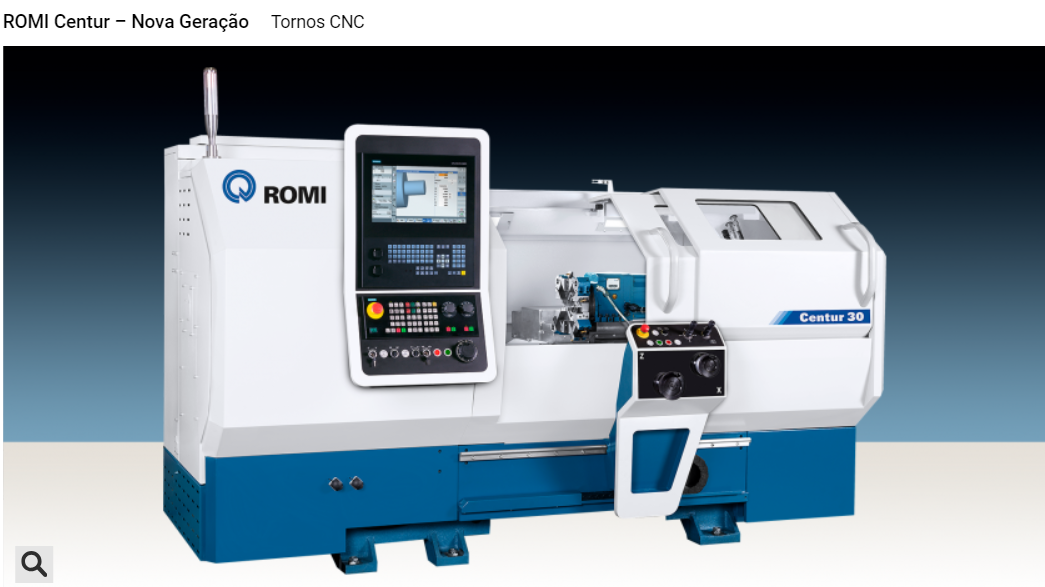
\includegraphics[width=0.48 \linewidth]{figs/romi_cnc.png}
    \caption{Imagem torno manual e CNC \cite{m:figs_tornos}}
    \label{fig:tornos}
\end{figure}

A Figura \ref{fig:tipo_usinagem} ilustra os principais métodos utilizados na manufatura na indústria, evidenciando que, muitas vezes, mais de uma atividade pode ser empregada para desenvolver uma determinada peça. Além disso, há peças que são inicialmente confeccionadas em formas, por meio de processos como estampagem ou fundição, e que posteriormente podem passar por acabamentos finais, como torneamento e fresamento.

\begin{figure}[h!]
    \centering
    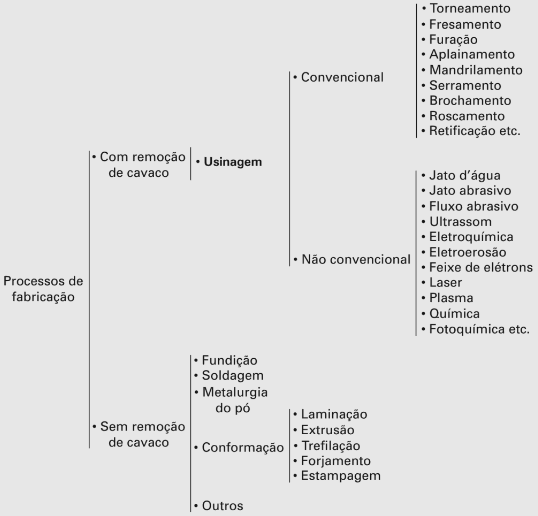
\includegraphics[width=0.75\linewidth]{figs/usinagem_tipos.png}
    \caption{Arvore fabricação de peças \cite{b:usinagem_2015} }
    \label{fig:tipo_usinagem}
\end{figure}

Graças à terceira revolução industrial, o sistema de usinagem avançou consideravelmente. Com o advento da informática, foi possível desenvolver tornos com comando numérico computadorizado, conhecidos como tornos CNC, conforme ilustrado Figura \ref{fig:tornos} imagem da direita. Para o desenvolvimento de peças, é fundamental criar um esquema de instruções, que pode ser elaborado por meio de softwares de \textit{Computer Aided Design  Computer Aided Manufacturing} (CAD-CAM) ou Solid-CAM na versão 3D, permitindo a criação do projeto da peça. Posteriormente, esses programas processa em esquema para a linguagem G-CODE, que é a linguagem padrão utilizada pelos tornos CNC para controlar todos os movimentos da máquina. Além disso, esses sistemas estão equipados com mecanismos de segurança que interrompem as operações em caso de falhas mecânicas, de hardware ou de software \mbox{\cite{a:torno_cnc_2022}.}

\section{Tecnologias para desenvolvimento web}
\label{sec:tecnologia_web}

Quando um usuário acessa um navegador e insere um endereço válido na internet, o navegador carrega um site específico, que, neste caso, corresponde a uma página ou sistema. Vários fatores estão envolvidos na determinação da página web a ser carregada, pois o processo se inicia com requisições de serviços. Essas requisições são essenciais para a comunicação entre o navegador e os servidores, permitindo que os dados sejam transferidos e a página desejada seja exibida ao usuário

Assim, para que máquinas e humanos, ou apenas máquinas, possam trocar informações, faz-se necessário a utilização de modelos e protocolos que padronizem o processo de envio e recebimento de dados. Nesse sentido, a web é constituída por um conjunto de pacotes organizados em uma estrutura hierárquica, que orienta os métodos de verificação para que não haja erros na transmissão. De modo que a comunicação, por sua vez, é realizada por meio de interfaces de programação, utilizando protocolos como o \textit{Hypertext Transfer Protocol} (HTTP), \textit{Hypertext Transfer Protocol Secure} (HTTPS) e \textit{File Transfer Protocol} (FTP), entre outros \mbox{\cite{b:redes_2017}.}

Por meio desses formatos e métodos, as páginas da web emprega \textit{Uniform Resource Locator} (URL), que converte \textit{World Wide Web} (WWW) em IP de domínios com o auxilio \textit{Domain Name System} (DNS) que realiza essa codificação. Assim, o navegador recebe esse endereço e o transmite para seus nós, realizando saltos através de roteadores que verificam quais rotas devem ser seguidas para levar a solicitação em menor tempo do cliente ao servidores e depois podem optar por rotas alternativas mais viáveis para retornar as solicitações \mbox{\cite{b:redes_2017}.}

Após estabelecer todos os mecanismos de comunicação necessários para a solicitação das informações, é essencial utilizar uma linguagem de marcação juntamente com uma linguagem de programação que contenha a lógica do sistema, permitindo o desenvolvimento do ambiente pode ser um site, blog ou um sistema web, havendo assim classificação como no back-end e front-end.

Dessa forma, o \textit{Hypertext Markup Language} (HTML) oferece a estrutura visual e esquemática essencial para que o usuário possa visualizar e interagir com o sistema, o HTML encontra se na sua quinta versão. Para aplicar estilizações, o \textit{Cascading Style Sheets} (CSS) proporciona melhorias visuais que formatam e facilitam a manutenção sempre que um elemento precisa de uma nova apresentação, de modo que framework mais utilizado é Bootstrap que está na sua quinta versão, que já contém uma estrutura estabelecidas basta conhecer a sintaxe para declara las nas tags do HTML. Por outro lado, para as máquinas, são suficientes conjuntos de protocolos, métodos, parâmetros e regras que organizam o envio e o recebimento das solicitações entre elas e o servidor, há bibliotecas ou APIs que possibilitam essa interação de trafego de dados na rede \mbox{\cite{a:api_redes_industria_v4_2024}.}

Para implementar a lógica e desenvolver métodos como \textbf{Create}, \textbf{Update} e \textbf{Delete}, é necessária uma linguagem de programação web, que podem ser da linguagem Java, PHP, Python, entre outras opções e atualmente há suporte para linguagem JavaScript que realiza função lógica para desenvolver sistema. Assim, dependendo dessa opção do desenvolvimento da programação, há frameworks que garantam uma estrutura padrão já implementadas com rotinas mais comuns. Para o PHP por exemplo pode ser Codeigniter.

O CodeIgniter é um framework para o desenvolvimento de aplicações web. O objetivo deste framework é agilizar o processo de desenvolvimento por meio de bibliotecas nativas, permitindo a integração de novas bibliotecas conforme necessário, utilizando o Composer. Ele é projetado para criar aplicações mais enxutas, com um menor tempo de configuração para iniciar um projeto, uma programação menos restritiva e a possibilidade de utilizar linhas de comando para o desenvolvimento \mbox{\cite{b:codeigniter4_2020}.}

A versão 4 do CodeIgniter introduziu o componente Spark, que facilita a criação de diversos elementos, incluindo a configuração do banco de dados — que, neste projeto, utilizará MySQL — até o desenvolvimento de controllers e models da aplicação. Para acessar mais informações, basta digitar o comando \textbf{php spark} no prompt de comando dentro do diretório da aplicação. Para detalhes adicionais e acesso à documentação, visite o site oficial do CodeIgniter \mbox{\cite{m:codeigniter4.5.4}.}
% ----------------------------------------------------------
% Metodologia
% ----------------------------------------------------------
\chapter{Metodologia}

As notas de rodapé são detalhadas pela NBR 14724:2011 na seção 5.2.1\footnote{As
notas devem ser digitadas ou datilografadas dentro das margens, ficando
separadas do texto por um espaço simples de entre as linhas e por filete de 5
cm, a partir da margem esquerda. Devem ser alinhadas, a partir da segunda linha
da mesma nota, abaixo da primeira letra da primeira palavra, de forma a destacar
o expoente, sem espaço entre elas e com fonte menor
\citeonline[5.2.1]{NBR14724:2011}.}\footnote{Caso uma série de notas sejam
criadas sequencialmente, o \abnTeX\ instrui o \LaTeX\ para que uma vírgula seja
colocada após cada número do expoente que indica a nota de rodapé no corpo do
texto.}\footnote{Verifique se os números do expoente possuem uma vírgula para
dividi-los no corpo do texto.}. 


% ---
\section{Tabelas}
% ---

\index{tabelas}A \autoref{tab-nivinv} é um exemplo de tabela construída em
\LaTeX.

\begin{table}[htb]
\ABNTEXfontereduzida
\caption[Níveis de investigação]{Níveis de investigação.}
\label{tab-nivinv}
\begin{tabular}{p{2.6cm}|p{6.0cm}|p{2.25cm}|p{3.40cm}}
  %\hline
   \textbf{Nível de Investigação} & \textbf{Insumos}  & \textbf{Sistemas de Investigação}  & \textbf{Produtos}  \\
    \hline
    Meta-nível & Filosofia\index{filosofia} da Ciência  & Epistemologia &
    Paradigma  \\
    \hline
    Nível do objeto & Paradigmas do metanível e evidências do nível inferior &
    Ciência  & Teorias e modelos \\
    \hline
    Nível inferior & Modelos e métodos do nível do objeto e problemas do nível inferior & Prática & Solução de problemas  \\
   % \hline
\end{tabular}
\legend{Fonte: \citeonline{van86}}
\end{table}

Já a \autoref{tabela-ibge} apresenta uma tabela criada conforme o padrão do
\citeonline{ibge1993} requerido pelas normas da ABNT para documentos técnicos e
acadêmicos.

\begin{table}[htb]
\IBGEtab{%
  \caption{Um Exemplo de tabela alinhada que pode ser longa
  ou curta, conforme padrão IBGE.}%
  \label{tabela-ibge}
}{%
  \begin{tabular}{ccc}
  \toprule
   Nome & Nascimento & Documento \\
  \midrule \midrule
   Maria da Silva & 11/11/1111 & 111.111.111-11 \\
  \midrule 
   João Souza & 11/11/2111 & 211.111.111-11 \\
  \midrule 
   Laura Vicuña & 05/04/1891 & 3111.111.111-11 \\
  \bottomrule
\end{tabular}%
}{%
  \fonte{Produzido pelos autores.}%
  \nota{Esta é uma nota, que diz que os dados são baseados na
  regressão linear.}%
  \nota[Anotações]{Uma anotação adicional, que pode ser seguida de várias
  outras.}%
  }
  \end{table}
\chapter{Resultados}

Neste capítulo, as seções foram subdivididas para melhorar o desenvolvimento da escrita da monografia. A divisão é a seguinte: a seção \ref{sec:Simplificando_trabalho} relembra as atividades relacionadas ao problema que o sistema visa melhorar, destacando a definição do escopo que foi implementado na versão inicial.

\section{Simplificação da proposta do trabalho}
\label{sec:Simplificando_trabalho}

Conforme descrito nas seções anteriores, este trabalho propõe o desenvolvimento de um sistema de ordem de serviço com foco em relatórios e dashboards, conforme indicado na seção \ref{sec:descobrir_problema} - Descobrir um problema, objetivando aprimorar o foco do gestor da V Tornos. Com base nessa análise, foram definidas nas atividades essenciais para criar um sistema inicial, conforme a seção \ref{sec:definir_escolpo} - Definir escopo do projeto, com o intuito de desenvolver um MVP. O interesse que em futuras versões, sejam realizadas atualizações que sigam as métricas estabelecidas na descoberta dos problemas e contemplem melhorias ou o acréscimo de novas atividades relacionadas aos propósitos identificado para desenvolver o sistema.

Com a catalogação da estrutura dos fatos que são salvas nos arquivos Excel dos respetivos clientes. Deu-se origem a base de dados vtornos. Onde é demonstrada inicialmente no capitulo \ref{sec:desenvolver_eer} - Desenvolver EER Workbench. Através dela, criou-se o modelo caso de uso demonstrado \ref{sec:esquematizar_uml}, onde correlacionada como as atividades. 
\section{Banco de dados}
\label{sec:banco_dados}
A utilização de um framework busca manter uma estrutura organizada e incluir ferramentas que contribuem para a agilidade e flexibilidade no desenvolvimento. Para o desenvolvimento do banco de dados, utilizou-se o componente \textbf{php spark db:create}, que gera o banco de dados \textbf{vtornos}. Para assegurar a padronização e evitar erros no banco de dados, o CodeIgniter oferece dois mecanismos: um para documentar a estrutura do banco de dados e outro para orientar as inserções dos dados. A primeira é desenvolvida com a migration que é uma forma de catalogar a estrutura que irá criar as tabelas do banco de dados que ficam armazenada no diretório app/Database/Migrations \cite{b:codeigniter4_2020} .

 Nesse processo, foram desenvolvidas 17 tabelas para a persistência e recuperação das informações, oferecendo uma solução estruturada e de fácil manutenção. Informações adicionais sobre essas tabelas são abordadas nas próximas seções do trabalho. A segunda etapa foca em manter uma estrutura padronizada para as inserções nas tabelas, conhecida como seeder. Basicamente, trata-se de um modelo que define uma classe de inserções para cada tabela específica. Esses seeders estão localizados no diretório app/Database/Seeds. A inserção de dados ocorre através da função run, que recebe todas as informações necessárias para gerar os registros na tabela referenciada.
\begin{figure}[hb!]
    \centering
    \begin{lstlisting}[style=phplisting]
        <?= $this->extend("layouts/tema_um") ?>
        <?= $this->section("style") ?>
            // IMPLEMENTAÇÕES EM CSS 
        <?= $this->endSection() />
        <?= $this->section("conteudo") ?>
            // IMPLEMENTAÇÃO DOS COMPOMENTES FORMULÁRIO, LISTA EM PHP E HTML
        <?= $this->endSection() ?>
        <?= $this->section("script") ?>
            // IMPLEMENTAÇÃO JAVASCRIPTS OU UTILITARIOS JQUERYS AJAX
        <?= $this->endSection() ?>
    \end{lstlisting}
    \caption{Estrutura para implementação das views no sistema V Tornos}
    \label{fig:layouts_tema_um}
\end{figure}
\begin{figure}
    \centering
    \begin{lstlisting}[style=phplisting]
        <!doctype html>
        <html lang="pt-br">
        <head>
            <title>Sistema V Tornos</title>
            
            <links>
            <?= $this->renderSection("style") ?>
        </head>
        <body>
            <nav>
            </nav>
            <?= $this->renderSection("conteudo") ?>

            <script>
            <?= $this->renderSection("script") ?>
        </body>
        </html>
    \end{lstlisting}
    \caption{Layout página central sistema V Tornos}
    \label{fig:tema_um}
\end{figure}
\section{Criando estrutura Layouts para sistema}
\label{sec:layouts}
A Figura \ref{fig:layouts_tema_um} apresenta a segmentação usada no desenvolvimento das views do sistema, com base na Figura \ref{fig:tema_um}. Essa abordagem tem como objetivo criar um espaço reservado, definido por \$this->renderSection(), que possui três seções: uma para componentes de \textbf{estilo}, dedicada a implementações em CSS; outra para o \textbf{conteúdo}, onde são inseridas as estruturas específicas para criação de formulários, tabelas de listagem ou geração dinâmica de gráficos; e, por último, a seção de \textbf{script}, que conterá códigos específicos em JavaScript.
\section{Sistema de Login}
\label{sec:login}
A Figura \ref{fig:UsuarioModel_orm} ilustra a estrutura básica para a configuração de Object Relational Mapping (ORM) no UsuarioModel. A linha 6 indica o nome da tabela que a classe irá instanciar, seguido pelo nome da chave primária, conforme está implementado no banco de dados. Na linha 9, é especificado que o retorno será no formato de objeto; por padrão, o comando make:model implementa o retorno em tipo array. O \$useSoftDeletes é uma opção para registrar as datas de criação e exclusão de um objeto, permitindo que, na prática, não haja exclusão efetiva na tabela. Para mais detalhes, consulte a documentação oficial \cite{m:codeigniter4.5.4}\footnote{\url{https://codeigniter.com/user_guide/models/model.html#usesoftdeletes}}. Por fim, é importante ressaltar que os atributos serão encapsulado pelo CodeIgniter e a linha 12 especifica quais colunas da tabela devem ser gerenciadas pelo framework nas tarefas essenciais do CRUD.
\begin{figure}[h!]
    \centering
    \begin{lstlisting}[style=phplisting]
        <?php
        namespace App\Models;
        use CodeIgniter\Model;
        class UsuarioModel extends Model
        {
            protected $table            = 'usuarios';
            protected $primaryKey       = 'idUsuario';
            protected $useAutoIncrement = true;
            protected $returnType       = 'object';
            protected $useSoftDeletes   = false;
            protected $protectFields    = true;
            protected $allowedFields    = [
                "nome",
                "email",
                "senha"
            ];
    \end{lstlisting}
    \caption{Estrutura ORM básica Classe Modelo Usuário}
    \label{fig:UsuarioModel_orm}
\end{figure}
Para gerenciar o login e logout, um controlador separado foi desenvolvido, o qual também manipula as informações do usuário. Assim, o UsuarioModel é utilizado tanto no UsuarioController, que manipula diretamente os dados do usuário, quanto no LoginController, que realiza as verificações necessárias para o acesso ao sistema. Essa estratégia garante uma gestão eficiente dos dados do usuário e das funcionalidades de autenticação.

A Figura \ref{fig:UsuarioModel_callbaks} mostra que é possível executar ações antes ou depois de inserir, atualizar, visualizar (usando as funções \textbf{first}, \textbf{find} e \textbf{findAll}) e excluir dados. Nesse contexto, a função hash senha foi desenvolvida para criptografar senhas em duas situações específicas: antes da inserção de um novo registro de usuário e ao atualizar uma senha existente. Além disso, é importante usar métodos nativos do PHP para verificar senhas, utilizando password verify, como ilustrado na linha 13 da Figura \ref{cod:loginController}. Com essa implementação, é possível aplicar um filtro para garantir a proteção necessária. Essa abordagem está documentada \ref{sec:Sprint_login} Sprint 5 - REALIZAR MECANISMO DE LOGIN, que descreve os dois métodos que podem ser implementados, conforme mostrado na Figura \ref{cod:AuthFilter}.
\begin{figure}
    \centering
    \begin{lstlisting}[style=phplisting]
        public function onLogin(){
        $validate = $this->validate([
            "email" => "required|valid_email",
            "senha" => "required"
        ]);
        if(!$validate){
            return redirect()->back()->with("errors", $this->validator->getErrors());
        }else{
            $login = $this->usuario->where("email", $this->request->getPost("email"))->first();
            if(!$login){
                return redirect()->back()->with("infoError", "Verifique suas credenciais e tente novamente!");
            }
            if(!password_verify($this->request->getPost("senha"), $login->senha)){
                return redirect()->back()->with("infoError", "Verifique suas credenciais e tente novamente!");
            }
            unset($login->senha);
            session()->set("login",$login);
            return redirect()->route("home.principal");
        }
    }
    \end{lstlisting}
    \caption{Implementação do método de logar}
    \label{cod:loginController}
\end{figure}
\begin{figure}[hb!]
    \centering
    \begin{lstlisting}[style=phplisting]
  public function before(RequestInterface $request, $arguments = null)
    {
        if(!session()->has("login")){
            return redirect()->route("login.tela");
        }
    }
    public function after(RequestInterface $request, ResponseInterface $response, $arguments = null)
    {
        //
    }
    \end{lstlisting}
    \caption{Filtro para verificar autenticação no sistema}
    \label{cod:AuthFilter}
\end{figure}
\begin{figure}
    \centering
    \begin{lstlisting}[style=phplisting]
        // TRECHO DE CÓDIGO USUARIOMODEL
        // Callbacks
        protected $allowCallbacks = true;
        protected $beforeInsert   = ["hash_senha"];
        protected $afterInsert    = [];
        protected $beforeUpdate   = ["hash_senha"];
        protected $afterUpdate    = [];
        protected $beforeFind     = [];
        protected $afterFind      = [];
        protected $beforeDelete   = [];
        protected $afterDelete    = [];

        public function hash_senha(array $data){
        $data["data"]["senha"] = password_hash($data["data"]["senha"], PASSWORD_DEFAULT);
        //var_dump($data);die;
        return $data;
        }
    }
\end{lstlisting}
\caption{Funções callbaks para criptografar senha}
\label{fig:UsuarioModel_callbaks}
\end{figure}
\section{Módulo para controle de maquinários de ofertas de serviços}
\label{}
% ----------------------------------------------------------
% Conclusão
% ----------------------------------------------------------
\chapter{Conclusão ou Considerações Finais}

Parte do texto que apresenta resultados correspondentes aos objetivos ou 
hipóteses levantadas na introdução e o produto final desenvolvido. 

Descreve, de forma resumida, o que se aprendeu sobre o tema, e pode até 
mesmo apresentar propostas de seguimento do assunto estudado. Deve estar 
coerente com o desenvolvimento e relacionado à introdução. Pode ainda estabelecer 
relações com outros fatos referentes à mesma matéria. 

Texto texto texto texto texto texto texto texto texto texto texto texto texto texto 
texto texto texto texto texto texto texto texto texto texto texto texto texto texto texto 
texto texto texto texto texto texto texto texto texto texto texto texto texto texto texto 
texto texto texto texto texto texto texto texto texto texto texto texto texto texto texto 
texto texto texto texto texto texto texto texto texto texto texto texto texto texto texto 
texto texto texto. 

Texto texto texto texto texto texto texto texto texto texto texto texto texto texto 
texto texto texto texto texto texto texto texto texto texto texto texto texto texto texto 
texto texto texto texto texto texto texto texto texto texto texto texto texto texto texto 
texto texto texto texto texto texto texto texto texto texto texto texto texto texto texto 
texto texto. 

Texto texto texto texto texto texto texto texto texto texto texto texto texto texto 
texto texto texto texto texto texto texto texto texto texto texto texto texto texto texto 
texto texto texto texto texto texto texto texto texto texto texto texto texto texto texto 
texto texto texto texto texto texto texto texto texto texto texto texto texto texto texto 
texto texto texto texto texto texto texto texto texto texto texto texto texto texto texto 
texto texto texto. 

Texto texto texto texto texto texto texto texto texto texto texto texto texto texto 
texto texto texto texto texto texto texto texto texto texto texto texto texto texto texto 
texto texto texto texto texto texto texto texto texto texto texto texto texto texto texto 
texto texto texto texto texto texto texto texto texto texto texto texto texto texto texto 
texto texto texto texto texto texto texto texto texto texto texto texto texto texto texto 
texto texto texto.
% ----------------------------------------------------------
% Trabalhos Futuros
% ----------------------------------------------------------

%% Para tornar os trabalhos futuros um capítulo a parte, use \chapter{Trabalhos Futuros}
\section{Trabalhos Futuros}



%% Finalizações para o PDF
\bookmarksetup{startatroot}

%% Elementos pós-textuais: Referências, Anexos, etc.
%% %%%%%%%%%%%%%%%%%%%%%%%%%%%%%%%%%%%%%%%%% %%
%% Elementos Pós Textuais
%% ----------------------
%% 
%% Segundo o manual do IFPI, eles devem ser os seguintes (nessa ordem):
%% 1. Referências (obrigatório)
%% 2. Glossário (opcional)
%% 3. Apêndice (opcional)
%% 4. Anexos (opcional)
%% 5. Índices (opcional)
%% %%%%%%%%%%%%%%%%%%%%%%%%%%%%%%%%%%%%%%%%% %%

%% Indica ao LaTeX que a partir deste ponto ficarão os elementos pós-textuais
\postextual

%% 01: Referências bibliográficas
%% Referências bibliográficas

\bibliography{bibliografia}

%% 02: Glossário
%% Glossário
%\glossary

%% 03: Apêndices
%% Apêndices

%\begin{apendicesenv}
%
%%% Imprime uma página indicando o início dos apêndices (opcional, comente para retirar)
%\partapendices
%
%%% Cada Capítulo será um apêndice
%\chapter{Este será o apêndice A}
%Lorem ipsum dolor sit amet, consectetur adipiscing elit. Praesent congue, turpis quis rutrum fringilla, lacus lorem faucibus diam, sit amet viverra urna quam sed metus. Pellentesque quis eros ex. Nullam vel ante rutrum eros placerat egestas. Morbi volutpat sapien elementum tincidunt fringilla. Class aptent taciti sociosqu ad litora torquent per conubia nostra, per inceptos himenaeos. Sed rutrum vestibulum bibendum. Sed tincidunt, magna sit amet tempor tincidunt, turpis neque blandit eros, a tincidunt felis mauris vitae est. Aliquam sit amet placerat risus. Nunc eget est pulvinar est tristique convallis sit amet vel risus. Maecenas turpis nisl, blandit ac porttitor non, ultrices id est. Cras eleifend nulla ut condimentum ullamcorper. Quisque at gravida massa, fringilla varius sapien. Nulla ullamcorper mauris vel ipsum elementum, vel tincidunt ante pretium. Ut iaculis nunc ex, vitae elementum ante efficitur non. Pellentesque venenatis tristique odio, nec volutpat dui dapibus sit amet. Maecenas eu velit at arcu hendrerit sagittis vel a odio.
%
%Nulla gravida metus at gravida ultricies. Nulla auctor id mi id suscipit. Proin vestibulum metus non eros feugiat, ac blandit diam vestibulum. Sed in arcu eget mauris rhoncus semper. Integer dignissim dui quis massa vestibulum, luctus ultrices metus mollis. Sed aliquam leo hendrerit lacus ultricies efficitur. Praesent quis quam sed lorem tincidunt fringilla non interdum odio. Phasellus vel enim mattis, tempor arcu ut, pulvinar est. Sed ut tempus est. Fusce erat nisi, scelerisque quis tellus sit amet, lacinia sagittis libero. Sed ultrices odio ipsum, ut vestibulum nulla auctor in.
%
%
%
%
%
%\chapter{Este será o apêndice B}
%Lorem ipsum dolor sit amet, consectetur adipiscing elit. Integer malesuada elit vel lacus fringilla, in luctus orci finibus. Praesent eget augue et enim luctus cursus ut ac nisl. In lobortis tellus non mauris euismod, tempus hendrerit nisi euismod. Integer id magna sapien. Nunc urna magna, consequat sed vehicula quis, convallis non justo. Aliquam risus dolor, viverra quis dignissim eget, convallis id sapien. Ut id turpis suscipit, mollis quam sed, lacinia lacus. Donec ac nulla dui.
%
%
%\end{apendicesenv}

%% 04: Anexos
%% Anexos
\begin{anexosenv}

%% Imprime uma página indicando o início dos anexos (opcional, comente para retirar)
%\partanexos

% Exemplo de inclusão
% \input{pos-textual/anexo} 
\chapter{TRECHO DA CARTA DE PERO VAZ DE CAMINHA} \label{anexo:a}
\vspace{-2cm}
\begin{figure}[H]
	\caption*{}
	\begin{center}
	    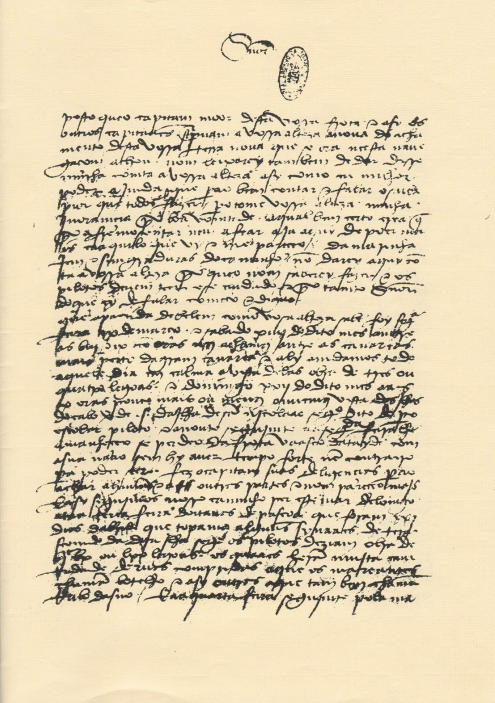
\includegraphics[scale=1.0]{imagens/carta_pero_vaz.png}
	\end{center}
	
\end{figure}


\end{anexosenv}

%% 05: Índices
%% Índices
%\phantompart \printindex

%% Capa do CD (opcional)
%%% Isso aqui cria a capa do CD, no final do documento :)
\newpage
\thispagestyle{empty}
\begin{center}
\covers[{\vspace{1.5cm} \Large \MakeUppercase{Curso de \imprimirnomedocurso} \\ \vspace{1cm} \textbf{\imprimirautor} \\ \vspace{0.5cm} {TÍTULO: \imprimirtitulo}}]{
	{\vspace{1.5cm} 
\includegraphics[scale=0.25]{imagens/ifpi.pdf} \\ \vspace{1cm} \MakeUppercase{Curso de \imprimirnomedocurso} \\ \vspace{1cm} {\textbf{\imprimirautor}} \\ \vspace{0.3cm} {TÍTULO: \imprimirtitulo} \\ \vspace{1.5cm} \MakeUppercase{\imprimirlocal} \par \imprimirdata}
}{
	\MakeUppercase{\tiny \imprimirtitulo}
}
\end{center}

\end{document}